\documentclass{standalone}
\usepackage{tikz}
\usetikzlibrary{patterns, positioning}


\begin{document}
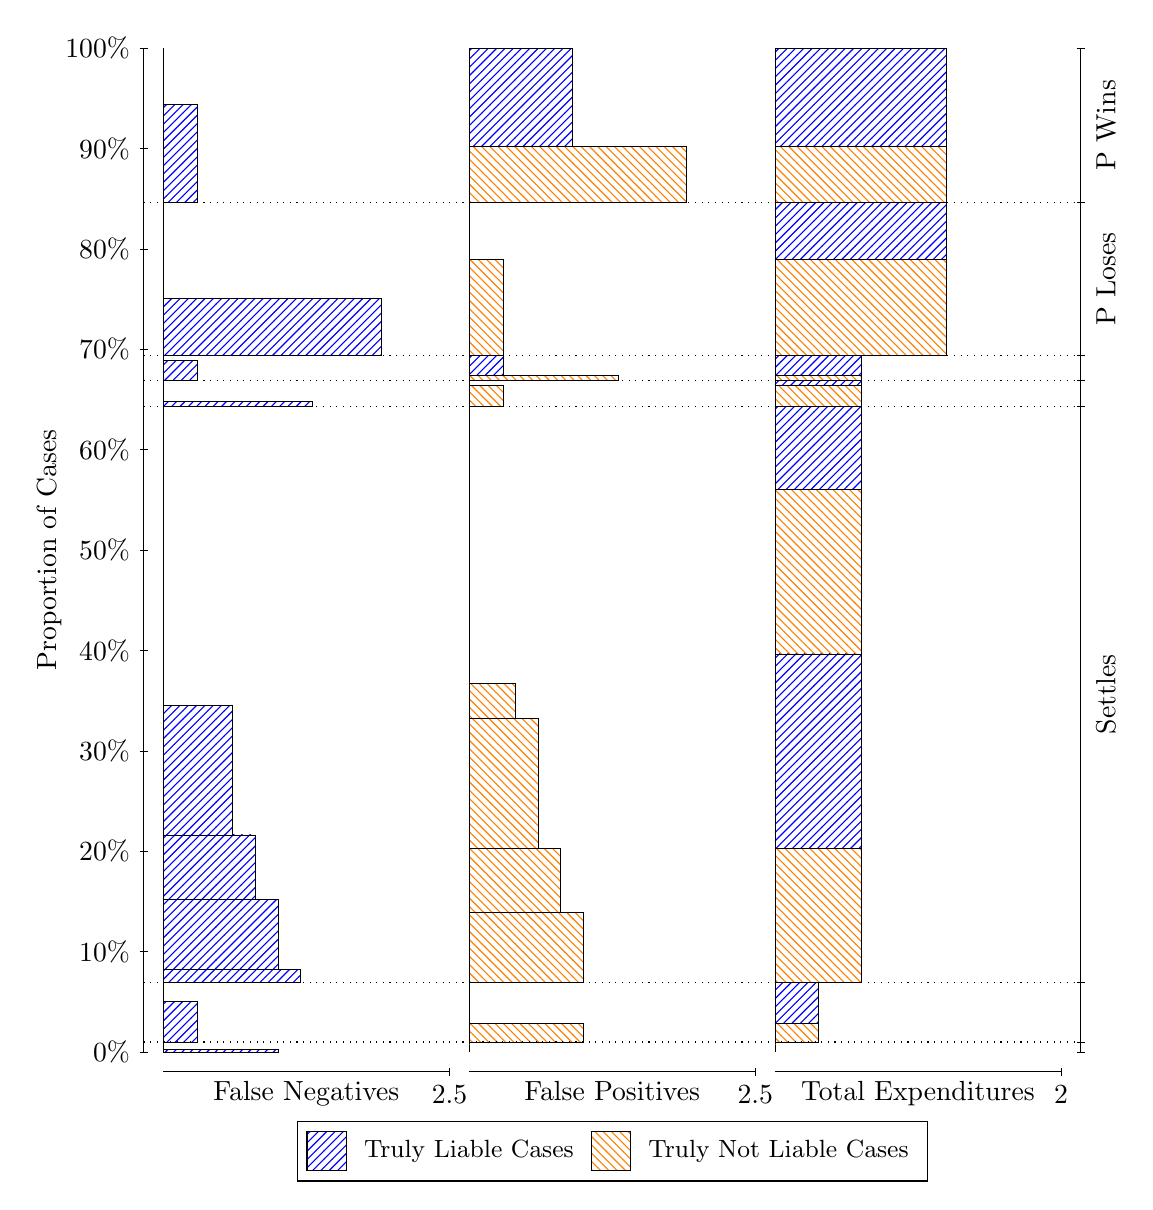
\begin{tikzpicture}
\draw[black, very thin] (1.5,1.75) -- (1.5,14.5);
\node[rotate=90, text=black, anchor=center] at (0.3, 8.125) {Proportion of Cases};
\draw[black, very thin] (1.45,1.75) -- (1.55,1.75);
\node[text=black, anchor=east] at (1.45, 1.75) {0\%};
\draw[black, very thin] (1.45,3.025) -- (1.55,3.025);
\node[text=black, anchor=east] at (1.45, 3.025) {10\%};
\draw[black, very thin] (1.45,4.3) -- (1.55,4.3);
\node[text=black, anchor=east] at (1.45, 4.3) {20\%};
\draw[black, very thin] (1.45,5.575) -- (1.55,5.575);
\node[text=black, anchor=east] at (1.45, 5.575) {30\%};
\draw[black, very thin] (1.45,6.85) -- (1.55,6.85);
\node[text=black, anchor=east] at (1.45, 6.85) {40\%};
\draw[black, very thin] (1.45,8.125) -- (1.55,8.125);
\node[text=black, anchor=east] at (1.45, 8.125) {50\%};
\draw[black, very thin] (1.45,9.4) -- (1.55,9.4);
\node[text=black, anchor=east] at (1.45, 9.4) {60\%};
\draw[black, very thin] (1.45,10.675) -- (1.55,10.675);
\node[text=black, anchor=east] at (1.45, 10.675) {70\%};
\draw[black, very thin] (1.45,11.95) -- (1.55,11.95);
\node[text=black, anchor=east] at (1.45, 11.95) {80\%};
\draw[black, very thin] (1.45,13.225) -- (1.55,13.225);
\node[text=black, anchor=east] at (1.45, 13.225) {90\%};
\draw[black, very thin] (1.45,14.5) -- (1.55,14.5);
\node[text=black, anchor=east] at (1.45, 14.5) {100\%};

\draw[black, very thin] (13.4,1.75) -- (13.4,14.5);
\draw[black, very thin] (13.35,1.75) -- (13.45,1.75);
\node[anchor=west] at (13.35, 1.75) {};
\draw[black, very thin] (13.35,1.8766) -- (13.45,1.8766);
\node[anchor=west] at (13.35, 1.8766) {};
\draw[black, very thin] (13.35,2.6331) -- (13.45,2.6331);
\node[anchor=west] at (13.35, 2.6331) {};
\draw[black, very thin] (13.35,9.9518) -- (13.45,9.9518);
\node[anchor=west] at (13.35, 9.9518) {};
\draw[black, very thin] (13.35,10.275) -- (13.45,10.275);
\node[anchor=west] at (13.35, 10.275) {};
\draw[black, very thin] (13.35,10.598) -- (13.45,10.598);
\node[anchor=west] at (13.35, 10.598) {};
\draw[black, very thin] (13.35,12.537) -- (13.45,12.537);
\node[anchor=west] at (13.35, 12.537) {};
\draw[black, very thin] (13.35,14.5) -- (13.45,14.5);
\node[anchor=west] at (13.35, 14.5) {};

\draw[black, very thin, pattern color=blue, pattern=north east lines] (1.75,1.75) rectangle (3.2033,1.7848);
\draw[black, very thin, pattern color=orange, pattern=north west lines] (1.75,1.7848) rectangle (1.75,1.8766);
\draw[black, very thin, pattern color=blue, pattern=north east lines] (1.75,1.8766) rectangle (2.186,2.3969);
\draw[black, very thin, pattern color=orange, pattern=north west lines] (1.75,2.3969) rectangle (1.75,2.6331);
\draw[black, very thin, pattern color=blue, pattern=north east lines] (1.75,2.6331) rectangle (3.494,2.8028);
\draw[black, very thin, pattern color=blue, pattern=north east lines] (1.75,2.8028) rectangle (3.2033,3.6898);
\draw[black, very thin, pattern color=blue, pattern=north east lines] (1.75,3.6898) rectangle (2.9127,4.5076);
\draw[black, very thin, pattern color=blue, pattern=north east lines] (1.75,4.5076) rectangle (2.622,6.1562);
\draw[black, very thin, pattern color=orange, pattern=north west lines] (1.75,6.1562) rectangle (1.75,9.9518);
\draw[black, very thin, pattern color=blue, pattern=north east lines] (1.75,9.9518) rectangle (3.6393,10.015);
\draw[black, very thin, pattern color=orange, pattern=north west lines] (1.75,10.015) rectangle (1.75,10.275);
\draw[black, very thin, pattern color=blue, pattern=north east lines] (1.75,10.275) rectangle (2.186,10.535);
\draw[black, very thin, pattern color=orange, pattern=north west lines] (1.75,10.535) rectangle (1.75,10.598);
\draw[black, very thin, pattern color=blue, pattern=north east lines] (1.75,10.598) rectangle (4.5113,11.322);
\draw[black, very thin, pattern color=orange, pattern=north west lines] (1.75,11.322) rectangle (1.75,12.537);
\draw[black, very thin, pattern color=blue, pattern=north east lines] (1.75,12.537) rectangle (2.186,13.787);
\draw[black, very thin, pattern color=orange, pattern=north west lines] (1.75,13.787) rectangle (1.75,14.5);
\draw[black, very thin, pattern color=orange, pattern=north west lines] (5.6333,1.75) rectangle (5.6333,1.8419);
\draw[black, very thin, pattern color=blue, pattern=north east lines] (5.6333,1.8419) rectangle (5.6333,1.8766);
\draw[black, very thin, pattern color=orange, pattern=north west lines] (5.6333,1.8766) rectangle (7.0867,2.1129);
\draw[black, very thin, pattern color=blue, pattern=north east lines] (5.6333,2.1129) rectangle (5.6333,2.6331);
\draw[black, very thin, pattern color=orange, pattern=north west lines] (5.6333,2.6331) rectangle (7.0867,3.5201);
\draw[black, very thin, pattern color=orange, pattern=north west lines] (5.6333,3.5201) rectangle (6.796,4.3379);
\draw[black, very thin, pattern color=orange, pattern=north west lines] (5.6333,4.3379) rectangle (6.5053,5.9866);
\draw[black, very thin, pattern color=orange, pattern=north west lines] (5.6333,5.9866) rectangle (6.2147,6.4287);
\draw[black, very thin, pattern color=blue, pattern=north east lines] (5.6333,6.4287) rectangle (5.6333,9.9518);
\draw[black, very thin, pattern color=orange, pattern=north west lines] (5.6333,9.9518) rectangle (6.0693,10.212);
\draw[black, very thin, pattern color=blue, pattern=north east lines] (5.6333,10.212) rectangle (5.6333,10.275);
\draw[black, very thin, pattern color=orange, pattern=north west lines] (5.6333,10.275) rectangle (7.5227,10.338);
\draw[black, very thin, pattern color=blue, pattern=north east lines] (5.6333,10.338) rectangle (6.0693,10.598);
\draw[black, very thin, pattern color=orange, pattern=north west lines] (5.6333,10.598) rectangle (6.0693,11.814);
\draw[black, very thin, pattern color=blue, pattern=north east lines] (5.6333,11.814) rectangle (5.6333,12.537);
\draw[black, very thin, pattern color=orange, pattern=north west lines] (5.6333,12.537) rectangle (8.3947,13.25);
\draw[black, very thin, pattern color=blue, pattern=north east lines] (5.6333,13.25) rectangle (6.9413,14.5);
\draw[black, very thin, pattern color=orange, pattern=north west lines] (9.5167,1.75) rectangle (9.5167,1.8419);
\draw[black, very thin, pattern color=blue, pattern=north east lines] (9.5167,1.8419) rectangle (9.5167,1.8766);
\draw[black, very thin, pattern color=orange, pattern=north west lines] (9.5167,1.8766) rectangle (10.062,2.1129);
\draw[black, very thin, pattern color=blue, pattern=north east lines] (9.5167,2.1129) rectangle (10.062,2.6331);
\draw[black, very thin, pattern color=orange, pattern=north west lines] (9.5167,2.6331) rectangle (10.607,4.3379);
\draw[black, very thin, pattern color=blue, pattern=north east lines] (9.5167,4.3379) rectangle (10.607,6.8044);
\draw[black, very thin, pattern color=orange, pattern=north west lines] (9.5167,6.8044) rectangle (10.607,8.8951);
\draw[black, very thin, pattern color=blue, pattern=north east lines] (9.5167,8.8951) rectangle (10.607,9.9518);
\draw[black, very thin, pattern color=orange, pattern=north west lines] (9.5167,9.9518) rectangle (10.607,10.212);
\draw[black, very thin, pattern color=blue, pattern=north east lines] (9.5167,10.212) rectangle (10.607,10.275);
\draw[black, very thin, pattern color=orange, pattern=north west lines] (9.5167,10.275) rectangle (10.607,10.338);
\draw[black, very thin, pattern color=blue, pattern=north east lines] (9.5167,10.338) rectangle (10.607,10.598);
\draw[black, very thin, pattern color=orange, pattern=north west lines] (9.5167,10.598) rectangle (11.697,11.814);
\draw[black, very thin, pattern color=blue, pattern=north east lines] (9.5167,11.814) rectangle (11.697,12.537);
\draw[black, very thin, pattern color=orange, pattern=north west lines] (9.5167,12.537) rectangle (11.697,13.25);
\draw[black, very thin, pattern color=blue, pattern=north east lines] (9.5167,13.25) rectangle (11.697,14.5);
\draw[black, dotted] (1.5,1.8766) -- (13.4,1.8766);
\draw[black, dotted] (1.5,2.6331) -- (13.4,2.6331);
\draw[black, dotted] (1.5,9.9518) -- (13.4,9.9518);
\draw[black, dotted] (1.5,10.275) -- (13.4,10.275);
\draw[black, dotted] (1.5,10.598) -- (13.4,10.598);
\draw[black, dotted] (1.5,12.537) -- (13.4,12.537);
\draw[black, very thin] (1.75,1.5) -- (5.3833,1.5);
\node[text=black, anchor=north] at (3.5667, 1.5) {False Negatives};
\draw[black, very thin] (5.3833,1.45) -- (5.3833,1.55);
\node[text=black, anchor=north] at (5.3833, 1.45) {2.5};

\draw[black, very thin] (5.6333,1.5) -- (9.2667,1.5);
\node[text=black, anchor=north] at (7.45, 1.5) {False Positives};
\draw[black, very thin] (9.2667,1.45) -- (9.2667,1.55);
\node[text=black, anchor=north] at (9.2667, 1.45) {2.5};

\draw[black, very thin] (9.5167,1.5) -- (13.15,1.5);
\node[text=black, anchor=north] at (11.333, 1.5) {Total Expenditures};
\draw[black, very thin] (13.15,1.45) -- (13.15,1.55);
\node[text=black, anchor=north] at (13.15, 1.45) {2};



\node[text=black, centered, rotate=90] at (13.72, 6.2925) {Settles};


\node[text=black, centered, rotate=90] at (13.72, 11.568) {P Loses};
\node[text=black, centered, rotate=90] at (13.72, 13.519) {P Wins};

\draw (7.449999999999999,1.5) node[draw=none] (baseCoordinate) {};
\begin{scope}[align=center]
        \matrix[scale=0.5, draw=black, below=0.5cm of baseCoordinate, nodes={draw}, column sep=0.1cm]{
            \node[rectangle, draw, minimum width=0.5cm, minimum height=0.5cm, pattern color=blue, pattern=north east lines] {}; &
            \node[draw=none, font=\small, text=black] (B) {Truly Liable Cases}; &
            \node[rectangle, draw, minimum width=0.5cm, minimum height=0.5cm, pattern color=orange, pattern=north west lines] {}; &
            \node[draw=none, font=\small, text=black] (B) {Truly Not Liable Cases}; \\
            };
\end{scope}

\end{tikzpicture}
\end{document}